\documentclass[12pt]{article}
\usepackage{latexsym}
\usepackage{amssymb,amsmath}
\usepackage[pdftex]{graphicx}
\usepackage{hyperref}
\usepackage{color}
\usepackage{tikz}

\topmargin = 0.1in \textwidth=5.7in \textheight=8.6in
\oddsidemargin = 0.2in \evensidemargin = 0.2in

\begin{document}
\begin{center}
COMPUTER SCIENCE 20, SPRING 2014 \\
\smallskip

Module \#5 (Induction Review)
\end{center}
Author: Steve Komarov\\
Reviewer: Nicholas Longenbaugh\\
Last modified: \today\\

\paragraph*{Executive Summary}

\begin{enumerate}

\item Ordinary Induction
\begin{itemize}
\item A {\em predicate} is the thing you are trying to prove.
\item Let $P(x)$ be a predicate and $m, n$ nonnegative integers.  If $P(m)$ is true and $P(n) \Rightarrow P(n+1)$ for all $n \ge m$, then $P(n)$ is true for all $n \ge m$.

\item To write a proof by induction, first you need to identify the proposition to be proven.  Then prove the base case, prove the inductive step (how you can get from the proposition holding for $n$ to the proposition holding for $n+1$), and the conclusion.  Be sure you identify properly the thing being inducted upon.
\end{itemize}

\item Strong Induction
\begin{itemize}
\item In simple terms, strong induction is similar to ordinary induction, except you use $P(0)$, $\ldots$, $P(n)$ instead of just $P(n)$ in order to prove $P(n+1)$.
\item Formally, the difference between ordinary and strong induction is:\\
Let $P(x)$ be a predicate and $m,n$ nonnegative integers.
    \begin{itemize}
    \item Ordinary Induction: If $P(m)$ is true and $P(n) \Rightarrow P(n+1)$\\ for all $n \geq m$, then $P(n)$ is true for all $n      \geq m$.
    \item Strong Induction: If $P(m)$ is true and\\ $P(m), P(m+1), \dots, P(n)$ together $\Rightarrow P(n+1)$\\
    for all $n \geq m$, then $P(n)$ is true for all $n \geq m$.
    \end{itemize}
\item Strong induction proofs begin with the identification of the proposition to be proven. The next step is to identify and verify the base case. Note that with strong induction there are often multiple base cases. Next comes the inductive step, where you show that the propositions truth for $0\ldots n$ entails its truth for $n+1$. Be sure to properly identify the proposition being inducted on.  
\item Note that sometimes you will need to break your inductive step into multiple cases.
\end{itemize}
\end{enumerate}

\paragraph*{Check-in questions}
\begin{enumerate}
\item Let P(n) mean "Postage of n cents can be made with only 4-cent and 7-cent stamps". For which of the following values of n is P(n) false?
\begin{enumerate}
    \item n=14
    \item n=15
    \item n=16
    \item n=17
    \item n=18
\end{enumerate}
\item Let P(n) mean "Postage of n cents can be made with only 4-cent and 7-cent stamps". Suppose that we want to prove by strong induction that P(n) is true for all $n>17$.  Which of the following base cases do we need to show? 
\begin{enumerate}
    \item P(0), P(1), P(2), P(3)
    \item P(14), P(15), P(16), P(17)
    \item P(17), P(18), P(19), P(20)
	\item P(18), P(19), P(20), P(21)

\end{enumerate}
\end{enumerate}

\pagebreak

\paragraph*{In-class Problems}
\begin{enumerate}

\item Using induction, prove that for all positive integers $n$ :
$$
\sum_{k=1}^{n}\frac{1}{k(k+1)}=\frac{n}{n+1}
$$

\item A tromino is an arrangement of three squares like the one shown below. It can be flipped and rotated in any direction. 

\begin{center}


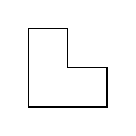
\begin{tikzpicture}[scale=0.5]

\draw (0,0) -- (2,0) -- (2,1) -- (1,1) -- (1,2) -- (0,2) -- (0,0);

\end{tikzpicture}
\end{center}


\begin{enumerate}
\item
 Prove by induction that every $2^n \times 2^n$ grid with one corner removed can be covered with trominos. Example:

\begin{center}


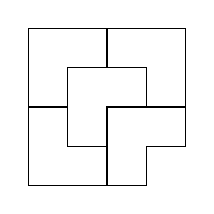
\begin{tikzpicture}[scale=0.5]

\draw (0,0) -- (3,0) -- (3,1) -- (4,1) -- (4,4) -- (0,4) -- (0,0);

\draw (2,0) -- (2,1) -- (1,1) -- (1,3) -- (3,3) -- (3,2) -- (2,2) -- (2,1);
\draw (0,2) -- (1,2);
\draw (2,4) -- (2,3);
\draw (3,2) -- (4,2);

\end{tikzpicture}
\end{center}

\item Explain how you can use the result from the previous part to prove that: 
\begin{center}
$2^{2n}-1$ is divisible by $3$, for all $n>0$
\end{center}

\end{enumerate}



\item You are putting together a jigsaw puzzle with $n \geq 1$ pieces. At each step you join together two matching pieces and produce a new (composite) piece. Prove by strong induction that no matter in which order you join the pieces, it takes $n-1$ steps to complete the puzzle. 

\item Consider the sequence $ a_1=1, a_2=3, ..., a_n=a_{n-1}+a_{n-2} $. Using strong induction prove that $ a_n\le \left( \frac{7}{4} \right) ^n $ for all positive integers $n$.


\item Prove the pigeonhole principle by induction. 

\end{enumerate}
\pagebreak



\end{document}
